%Version 3 December 2023
% See section 11 of the User Manual for version history
%
%%%%%%%%%%%%%%%%%%%%%%%%%%%%%%%%%%%%%%%%%%%%%%%%%%%%%%%%%%%%%%%%%%%%%%
%%                                                                 %%
%% Please do not use \input{...} to include other tex files.       %%
%% Submit your LaTeX manuscript as one .tex document.              %%
%%                                                                 %%
%% All additional figures and files should be attached             %%
%% separately and not embedded in the \TeX\ document itself.       %%
%%                                                                 %%
%%%%%%%%%%%%%%%%%%%%%%%%%%%%%%%%%%%%%%%%%%%%%%%%%%%%%%%%%%%%%%%%%%%%%

%%\documentclass[referee,sn-basic]{sn-jnl}% referee option is meant for double line spacing

%%=======================================================%%
%% to print line numbers in the margin use lineno option %%
%%=======================================================%%

%%\documentclass[lineno,sn-basic]{sn-jnl}% Basic Springer Nature Reference Style/Chemistry Reference Style

%%======================================================%%
%% to compile with pdflatex/xelatex use pdflatex option %%
%%======================================================%%

%%\documentclass[pdflatex,sn-basic]{sn-jnl}% Basic Springer Nature Reference Style/Chemistry Reference Style


%%Note: the following reference styles support Namedate and Numbered referencing. By default the style follows the most common style. To switch between the options you can add or remove “Numbered” in the optional parenthesis. 
%%The option is available for: sn-basic.bst, sn-vancouver.bst, sn-chicago.bst%  
 
%%\documentclass[pdflatex,sn-nature]{sn-jnl}% Style for submissions to Nature Portfolio journals
%%\documentclass[pdflatex,sn-basic]{sn-jnl}% Basic Springer Nature Reference Style/Chemistry Reference Style
\documentclass[pdflatex,sn-mathphys-num]{sn-jnl}% Math and Physical Sciences Numbered Reference Style 
%%\documentclass[pdflatex,sn-mathphys-ay]{sn-jnl}% Math and Physical Sciences Author Year Reference Style
%%\documentclass[pdflatex,sn-aps]{sn-jnl}% American Physical Society (APS) Reference Style
%%\documentclass[pdflatex,sn-vancouver,Numbered]{sn-jnl}% Vancouver Reference Style
%%\documentclass[pdflatex,sn-apa]{sn-jnl}% APA Reference Style 
%%\documentclass[pdflatex,sn-chicago]{sn-jnl}% Chicago-based Humanities Reference Style

%%%% Standard Packages
%%<additional latex packages if required can be included here>

\usepackage{graphicx}%
\usepackage{multirow}%
\usepackage{amsmath,amssymb,amsfonts}%
\usepackage{amsthm}%
\usepackage{mathrsfs}%
\usepackage[title]{appendix}%
\usepackage{xcolor}%
\usepackage{textcomp}%
\usepackage{manyfoot}%
\usepackage{booktabs}%
\usepackage{algorithm}%
\usepackage{algorithmicx}%
\usepackage{algpseudocode}%
\usepackage{listings}%
\usepackage{comment}
%%%%


%% as per the requirement new theorem styles can be included as shown below
\theoremstyle{thmstyleone}%
\newtheorem{theorem}{Theorem}%  meant for continuous numbers
%%\newtheorem{theorem}{Theorem}[section]% meant for sectionwise numbers
%% optional argument [theorem] produces theorem numbering sequence instead of independent numbers for Proposition
\newtheorem{proposition}[theorem]{Proposition}% 
%%\newtheorem{proposition}{Proposition}% to get separate numbers for theorem and proposition etc.

\theoremstyle{thmstyletwo}%
\newtheorem{example}{Example}%
\newtheorem{remark}{Remark}%

\theoremstyle{thmstylethree}%
\newtheorem{definition}{Definition}%

\raggedbottom
%%\unnumbered% uncomment this for unnumbered level heads

\begin{document}

\title[Article Title]{Bayesian Evidence of alternative models of P2X2 activation}

\author*[1]{\fnm{Luciano} \sur{Moffatt}}\email{lmoffatt@qi.fcen.uba.ar}
\author[2]{\fnm{Gustavo} \sur{Pierdominici-Sottile}}\email{gustavopierdominici@gmail.com }
%\equalcont{These authors contributed equally to this work.}

%\author[1,2]{\fnm{Third} \sur{Author}}\email{iiiauthor@gmail.com}
%\equalcont{These authors contributed equally to this work.}

\affil*[1]{\orgdiv{Instituto de Qu\'{i}mica F\'{i}sica de los Materiales, Medio Ambiente y Energ\'{i}a}, \orgname{  Consejo Nacional de Investigaciones Científicas y T\'{e}cnicas}, \orgname{Universidad de Buenos Aires} , \city{Buenos Aires}, \postcode{1428},  \country{Argentina}}

\affil[2]{\orgdiv{Departamento de Ciencia y Tecnolog\'{i}a, 
  Consejo Nacional de Investigaciones Científicas y T\'{e}cnicas} \orgname{Universidad Nacional de Quilmes}, \orgaddress{\street{S\'{a}enz Pe\~{n}a 352}, \city{Bernal}, \postcode{B1876BXD}, \state{Buenos Aires}, \country{Argentina}}}

%\affil[3]{\orgdiv{Department}, \orgname{Organization}, \orgaddress{\street{Street}, \city{City}, \postcode{610101}, \state{State}, \country{Country}}}

\begin{comment}
ESTAMOS 78 PALABRAS ENCIMA DE LO SUGERIDO
\end{comment}


\abstract{Ligand-activated receptors are essential for cellular signaling and represent significant therapeutic targets. Among these, the P2X receptor family, activated by ATP, plays a crucial role in various physiological processes, yet the molecular mechanisms governing its activation remain inadequately understood, particularly regarding the conformational dynamics between subunit interactions. Here, we demonstrate that ATP binding induces asymmetric conformational changes in the P2X receptor, specifically driving the rotation of the subunit bound by the lower body (LB), while the upper body (UP)-bound subunit remains stationary. We re-analyze previously published data from outside-out patch preparations of rP2X2 in response to ATP pulses of varying concentrations (0.2-10 mM) using a novel Bayesian algorithm that leverages kinetic information from response fluctuations. This analysis reveals that agonist binding promotes rotational shifts in the LB subunit 100 to 10,000 times more frequently than in the UP subunit. LB subunit rotation accelerates agonist binding and delays release, whereas UP subunit rotation slows both processes. Our findings elucidate distinct roles at the subunit interfaces: the UP subunit functions as an anchor, while LB subunit rotation enhances ATP binding energy and stabilizes the receptor in its active state. Once rotated, the UP subunit shields ATP, limiting its exchangeability and further stabilizing the binding site.

We anticipate that our Bayesian kinetic analysis will be instrumental in validating and refining the activation model presented here. This framework can be extended to investigate mutations, partial agonists, and other subunits. Furthermore, the notion of one subunit acting as an anchor while another serves as an allosterically active component may be applicable to other ligand-activated receptors. These insights could pave the way for developing innovative pharmaceutical agents targeting P2X receptors and related signaling pathways.
}




%%================================%%
%% Sample for structured abstract %%
%%================================%%

% \abstract{\textbf{Purpose:} As a guide the abstract should not exceed 200 words. Most journals do not set a hard limit however authors are advised to check the author instructions for the journal they are submitting to.
% 
% \textbf{Methods:} The abstract serves both as a general introduction to the topic and as a brief, non-technical summary of the main results and their implications. The abstract must not include subheadings (unless expressly permitted in the journal's Instructions to Authors), equations or citations. As a guide the abstract should not exceed 200 words. Most journals do not set a hard limit however authors are advised to check the author instructions for the journal they are submitting to.
% 
% \textbf{Results:} The abstract serves both as a general introduction to the topic and as a brief, non-technical summary of the main results and their implications. The abstract must not include subheadings (unless expressly permitted in the journal's Instructions to Authors), equations or citations. As a guide the abstract should not exceed 200 words. Most journals do not set a hard limit however authors are advised to check the author instructions for the journal they are submitting to.
% 
% \textbf{Conclusion:} The abstract serves both as a general introduction to the topic and as a brief, non-technical summary of the main results and their implications. The abstract must not include subheadings (unless expressly permitted in the journal's Instructions to Authors), equations or citations. As a guide the abstract should not exceed 200 words. Most journals do not set a hard limit however authors are advised to check the author instructions for the journal they are submitting to.}

\keywords{Bayesian Analysis, P2X receptors, Cellular Signaling}

\maketitle

\section{Introduction}\label{sec1}


Ligand-gated ion channels (LGICs) are multimeric membrane proteins that allow ions to cross the cell membrane in response to ligand binding \cite{p2x_cuerpo_humano}. These channels play critical roles in synaptic transmission, muscle contraction, and other physiological processes (add them), making them important targets in neuropharmacology \cite{p2x_drugs,therapeutic,p2x7_pharmacology}. LGIC families are classified based on their subunit composition and the location of ligand-binding sites. In pentameric Cys-loop receptors, the binding site is located at the interface between adjacent subunits, while in tetrameric glutamate receptors, it is within individual subunits. In trimeric P2X receptors, like Cys-loop receptors, the binding sites are located between subunits.

P2X receptors are the only LGICs for which high-resolution structures of both open and closed conformations are available \cite{cerrada_p2x,abierta_p2x}. These structures reveal that ATP binding triggers a rotational movement in all three subunits, leading to the separation of the transmembrane domains that form the pore, allowing ions to pass through. However, the intermediate states between these conformations remain unresolved. Understanding these intermediate states is essential for elucidating the mechanism of channel opening, which could inform the design of drugs that modulate P2X receptor function.

Two types of gating models have been proposed for P2X receptor activation: sequential rotation models, where subunits rotate one at a time to gradually open the pore, and synchronous models, where all subunits rotate together in a concerted motion. In sequential models, a key question arises about potential asymmetry: whether one subunit rotates first, specifically the subunit bound to the ATP by the Lower Body or the one bound by the Upper Body. Resolving this question is crucial for understanding the full activation mechanism of P2X receptors opening the door for a clever pharmacological design. 

In the case of P2X2 receptors, recordings of macroscopic currents in response to ultrashort (0.2 ms) ATP pulses provide valuable insights into the channel's activation process \cite {Moffatt_hume}. Previous models fitted to these data have proposed both sequential and synchronous gating schemes. However, early models incorrectly assumed intrasubunit binding sites akin to glutamate receptors, and no direct comparison of the evidence for the two gating models has been performed. 

Macrocurrents reflect the collective activity of numerous channels. The fluctuations in these currents contain valuable kinetic information. To analyze these fluctuations, we developed a novel algorithm, MacroIR, which improves upon the Macroscopic Recursive (MacroR) algorithm by accounting for finite integration times in voltage clamp recordings. MacroIR calculates the mean conductance and its variance over specified time intervals, providing a more accurate approximation of the likelihood function.

In this study, we applied MacroIR to our previously published recordings of ultrashort ATP pulses to investigate P2X2 receptor gating. We introduced new sequential gating schemes that take into account the inter-subunit binding sites and employed an affine-invariant Monte Carlo Markov chain (MCMC) algorithm to calculate posterior distributions and model evidence. Our results reveal that a sequential model with asymmetric allosteric coupling has a stronger evidence than either  symmetric sequential or synchronous models. Our study provides a novel framework for analyzing gating mechanisms in P2X2 receptors by combining advanced kinetic modeling with the MacroIR algorithm, offering new insights into receptor activation.


\section{Methods}\label{sec11}


\subsubsection{Markov model of the behavior of a single channel}

From the early days of single channel recordings its was clear that the channel was open and closed at irregular intervals in what seemed to be a stochastic process, what is unsurprising given the thermal fluctuations a macromolecule is exposed to. Therefore it was straightforward to model it as a Markov process of a finite number of states $k$, each representing a subset of the conformations of the whole protein. The Markov process cannot ascertain where the channel is at each moment of time but it provides a probability of finding the channel at each state defined by the state vector $\bold p$. It assumes a constant jump probability rate from one state $i$  to the other $j$, $k_{ij}$. The evolution of the probability of finding the channel in each state is set by the vector $\bold p$ - for a time lapse $t$ is defined by first order differential equation: 

\begin{equation}
\frac {d \bold p}{dt}(t) = \bold p(t) \cdot \bold Q (t)
\label{eq:eq1}
\end{equation}
where the elements off the diagonal of $\bold Q$ are the values $k_{ij}$ and the diagonal of $\bold Q$, $k_{ii}$ is defined as
\begin{align}
k_{ii}=- \sum_{j, j \neq i} k_{ij} \label{eq2}
\end{align}



The integration of Eq. \ref{eq:eq1} allow us to calculate the evolution of $ \bold p$
\begin{equation}
\bold p(t) = \bold p(0) \cdot \exp(\bold Q \cdot t)
\label{eq:eq2}
\end{equation}
 

The actual state of the Markov process is hidden, it is not observable. What is observable is the single current that each state generates. This is coded in the current vector $\bold \gamma$. 


\subsubsection{Bayesian model of instantaneous measurements of a single channel behavior}

Suppose now we made a one "instantaneous" current measurement y. We are told that the state
 probability is $p_{prior}$. We are told that the instrumental noise for each measurement has a variance of $\epsilon$. 
Then, we can obtain the posterior probability and the likelihood of measurement 
\begin{equation}
Lik=P(y_{obs})= \sum_i Normal (p_i \cdot \gamma_i - y_{obs}, \epsilon^2 ) 
\end{equation}

 and the posterior probability
\begin{equation}
p_{post} = p_i \cdot \frac {Normal(p_i \cdot \gamma_i -y, \epsilon)}{P(y_{obs})}
\end{equation}

now suppose we do another measurement after some time t. Then 

\begin{align}
p_{prior}(t) = p_{post}(0) \cdot \bold P  \nonumber \\
\bold P = \exp(\bold Q \cdot t)
\end{align}
\ 

and we can in the same way calculate the next posterior and Likelihood

The total logLikelihood is
\begin{equation}
logLik= \sum_i \log(Lik_i)
\end{equation}

 


\subsubsection{Bayesian model of time averaged measurements of a single channel behavior}
Suppose now that instead of an instantaneous measurement, we have the averaged current during the interval $t$. 
We have also the prior state $p_{prior}$ at the beginning of the interval t. We can also calculate the prior state probability at the end of the interval t, which is conditional to the probability state at the begining of the interval. Therefore, the joint state probability matrix P  of starting at state i and ending at state j is given by

\begin{equation}
\bold \Pi  = diag (\bold p) \cdot \bold P
\end{equation}

Now, we can obtain the likelihood of the average measurement and posterior distribution of P 
\begin{equation}
P(y_{obs}) =\sum_{ij} \Pi_{ij} \cdot Normal \left(y_obs-{\Pi_{ij} \cdot {\overline \Gamma}_{ij}} , \epsilon^2 + \sigma^2_{\overline{\Gamma} ij} \right)
\end{equation}



\begin{equation}
\Pi^{post}_{ij} = \frac {\Pi^{prior}_{ij} \cdot Normal \left (y_{obs}-{\Pi^{prior}_{ij} \cdot {\overline \Gamma}_{ij}} , \epsilon^2 + \sigma^2_{\overline{\Gamma}_{ij}} \right)}{P(y_{obs})}
\end{equation}




where $ {\overline \Gamma}_{ij}$  and $\sigma^2_{\overline{\Gamma}_{ij}}$ indicate the average current and variance of average current for starting at state $i$ and ending at state $j$. 

To complete the recursion we calculate the prior state for the beginning of the next interval is obtained just by row marginalization
\begin{equation}
p^{prior}_{j}(t_{n+1}) =\sum_i \Pi^{post}_{ij}(t_n)  
\end{equation}


. 
The growing cumulative log-likelihood of the whole measurement series is updated
\begin{equation}
logLikelihood \left(y^{obs}_{1 \dots n+1} \right) = logLikelihood (y^{obs}_{ 1 \dots n}) +log(P(y^{obs}_{n+1}))
\end{equation}


It is important to note that the distribution of the mean current is not normal. However, as long as the instrumental noise is much bigger than the gating noise, the approximation to a normal is reasonable. 

Calculation of the average current and average current variance. 
\begin{equation}
E(\Gamma_{ij}) = { \overline  \Gamma}_{ij} = {\frac {1} {t \cdot P_{ij}} } \cdot  \int_0^t \sum_k P_{ik}(\tau) \cdot \Gamma_k \cdot P_{kj}(t-\tau)\cdot d\tau 
\end{equation}

\begin{equation}
var({\overline  \Gamma}_{ij}) = E({\overline  \Gamma}_{ij}^2)- P_{ij} \cdot (E({\overline  \Gamma}_{ij}))^2
\end{equation}




\begin{equation}
E({\overline \Gamma}_{ij}^2) = {\frac {1} {t^2 \cdot P_{ij}} } \cdot  \int_0^t   \int_0^{t-\tau_1}   \sum_{k1`k2}P_{ik1}(\tau_1) \cdot \gamma_{k1} P_{k1`k2}(\tau_2) \cdot \gamma_{k2} \cdot P_{k2`j}(t-\tau_1-\tau_2)d\tau 
\end{equation}


\begin{equation}
{\overline \Gamma}_{i,j} = \frac{1}{P_ij}\sum_{k,n_1,n_2} V_{i n_1} \cdot  V^{-1}_{n_1 k} \cdot \gamma_k \cdot V_{k n_2} \cdot V^{-1}_{n_2 j} E_2(\lambda_{n_1} \cdot t, \lambda_{n_2} \cdot t) 
\end{equation}





\begin{equation}
E_2(x,y)= 
\begin{cases}
    \frac{\exp(x)-\exp(y)}{x-y},& x\neq y\\
    \exp(x),              & x=y
\end{cases}
\end{equation}


\begin{equation}
E_3(x,y,z)= 
\begin{cases}
    E_{111}(x,y,z),& x\neq y,y\neq z,z\neq x \\
    E_{12}(x,y,z), & x\neq y,x\neq z,y = z \\
    E_{12}(y,z,x), & y\neq z,y\neq x,z = x \\
    E_{12}(z,x,y), & z\neq x,z\neq y,x = y \\
   \frac {1}{2} \cdot \exp(x) , & x=y=z \\
  
\end{cases}
\end{equation}



\begin{equation}
E_{111}(x,y,z)= E_{1,11}(x, y, z) + E_{1,11}(y, x, z) +   E_{1,11}(z, y, x)
\end{equation}


\begin{equation}
E_{1,11}(x,y,z) = frac {exp(x)} { (x - y) cdot  (x - z)}
\end{equation}



\begin{equation}
\end{equation}






Going from single-channel to channel ensemble. 
When the only information we have on the ensemble of channels is the state probability vector, that indicates the probability for each individual channel of being in a particular state, a multinomial distribution would indicate the probability for each  possible distinct value of the state count vector. 
However, the posterior distribution of the ensemble state will depart from a multinomial and inverse correlations will appear for states with the same current. Although the channels be independent from each other, the information we have about them is not longer so. This is reminiscent to quantum entanglement. Therefor we need a way to describe the posterior probability. 
A safe and very expensive way is to build a vector, we call ensemble state vector, with all the possible combinations of state counts and apply bayes rule for each individual row. I call this the Microscopic Recursive Algorithm, which becomes computationally prohibitive very soon. 
This complete knowledge can be approximated by a mulivariate normal of the state count vector, that would be a Macroscopic approach. In this way the ensemble state distribution is approximated. Then the combination of 

In the MacroR algorithm, we considered the measurments as instantaneous and we consider just the instantaneous state of the ensemble, the mean probability state and  covariance probability state. It was shown that 

\begin{equation}
L_0= Normal \left (y^{obs}_0-y^{fit}_0, {\sigma^2}^{fit}_{0} \right)
\end{equation}


\begin{equation}
y^{fit}_0 = N_{ch} \cdot \mathbf \mu^{prior}_0 \cdot \mathbf \gamma
\end{equation}



\begin{equation}
{\sigma^2}^{fit}_{0}
= \epsilon^2 +N_{ch} \cdot {\mathbf \gamma}^{\mathrm{T}} \cdot \mathbf \Sigma^{prior}_0 \cdot \mathbf \gamma
\end{equation}

\begin{equation}
\mathbf \mu^{post}_0= \mathbf \mu^{prior}_0 + {\frac {y^{obs}_0 - y^{fit}_0}{{\sigma^2}^{fit}_0} }\cdot {\mathbf \gamma}^\mathrm{T} \cdot \mathbf \Sigma^{prior}_0 
\end{equation}

\begin{equation}
\mathbf \Sigma^{post}_0 = \mathbf \Sigma^{prior}_0 - {\frac {N}{{\sigma^2}^{fit}_0}}\cdot \mathbf \Sigma^{prior}_0 \cdot \mathbf \gamma \cdot {\mathbf \gamma}^\mathrm{T} \cdot \mathbf \Sigma^{prior}_0
\end{equation}

\begin{equation}
\mathbf \Sigma^{prior}_t= \mathrm{diag}(\mathbf \mu^{prior}_t ) + {\mathbf P(t)}^\mathrm{T} \cdot (\mathbf \Sigma^{post}_t- \mathbf \mu^{post}_t) \cdot \mathbf P( t)
\end{equation}

we can calculate the prior probability at time t
\begin{equation}
\mathbf \mu^{prior}_t = \mathbf \mu^{post}_0 \cdot \mathbf P(t)
\end{equation}

\begin{equation}
\mathbf \Sigma^{prior}_t= \mathrm{diag}(\mathbf \mu^{prior}_t ) + {\mathbf P(t)}^\mathrm{T} \cdot (\mathbf \Sigma^{post}_t- \mathbf \mu^{post}_t) \cdot \mathbf P( t)
\end{equation}



All these calculations can be used for Macroscopic Interval Recursive algorithm. The idea is that the description of the state considers now both the initial ensemble state and the final ensemble state during the measuring interval. 
So 

\begin{equation}
(\mu^{prior}_{t, t+ \Delta t})_{(i_t, i_{t+ \Delta t})} = (\mu^{prior}_{t})_{i_t}  \cdot P_{i_t \rightarrow i_{t+ \Delta t}}(\Delta t)
\end{equation}

\begin{multline}
(\Sigma^{prior}_{t,t+ \Delta t})_{(i_t, i_{t+ \Delta t})(j_t, j_{t+ \Delta t})} =
P_{i_t \rightarrow i_{t+ \Delta t}} \left((\Sigma^{prior}_{t})_{i_t ,j_t} - \delta_{i_t, j_t} \cdot (\mu^{prior}_t)_{i_t} \right)  \cdot P_{j_t \rightarrow j_{t+ \Delta t}} \\
+ \delta_{i_t, j_t} \cdot \delta_{i_{t+ \Delta t}, j_{t+ \Delta t}} \cdot (\mu^{prior}_t)_{i_t}\cdot P_{i_t \rightarrow i_{t+ \Delta t}} 
\end{multline}

we have the vectors 

\begin{equation}
({\overline \gamma}_{t,t+\Delta t })_{(i_t, i_{t+\Delta t})} = {\overline \Gamma}_{i_t,i_{t+\Delta t}}
\end{equation}

\begin{equation}
(\sigma^2{\overline \gamma}_{t,t+\Delta t })_{(i_t, i_{t+\Delta t})} = \sigma^2{\overline \Gamma}_{i_t,i_{t+\Delta t}}
\end{equation}

Lets now apply the MacroR formulae
\begin{equation}
L_{t, t+\Delta t}= Normal (y^{obs}_{t, t+\Delta t}-y^{fit}_{t, t+\Delta t}, {\sigma^{2}}^{fit}_{t, t+\Delta t}})
\end{equation}

\begin{equation}
y^{fit}_{t,t+\Delta t} = N_{ch} \cdot \mathbf \mu^{prior}_{t,t+\Delta t} \cdot \mathbf \gamma_{t,t+\Delta t}
\end{equation}

\begin{equation}
{\sigma^2}^{fit}_{t, t+\Delta t}
= \epsilon^2_{t, t+\Delta t} +N_{ch} \cdot {\mathbf \gamma}^{\mathrm{T}}_{t, t+\Delta t} \cdot \mathbf \Sigma^{prior}_{t, t+\Delta t} \cdot \mathbf \gamma_{t, t+\Delta t}
+ N_{ch} \cdot \mathbf \mu^{prior}_{t, t+\Delta t} \cdot {\sigma \mathbf  \Gamma}_{t, t+\Delta t}
\end{equation}

\begin{multline}
\mathbf \mu^{prior}_{t,t+\Delta t} \cdot \mathbf \gamma_{t,t+\Delta t} =
\sum_{i_t, i_{t+ \Delta t}} {(\mu^{prior}_{t})_{i_t}  \cdot P_{i_t \rightarrow i_{t+ \Delta t}}(\Delta t) \cdot ({\overline \Gamma_{t,t + \Delta t}})_{i_t \rightarrow i_{t+\Delta t}}}\\= \mathbf \mu^{prior}_t \cdot  \overline {\mathbf \gamma}_{t, t+\Delta t}
\end{multline}






so, the expected current does not depend on the end state, only on the state at the beginning of the interval and the expected current throughout the interval conditional on starting on a given state. 

\begin{multline}
    {\mathbf \gamma}^{\mathrm{T}}_{t, t+\Delta t} \cdot \mathbf \Sigma^{prior}_{t, t+\Delta t} \cdot \mathbf \gamma_{t, t+\Delta t}= \\
 \sum_{i_t, i_{t +\Delta t},j_t, j_{t +\Delta t}}
 ({\overline \Gamma_{t,t + \Delta t}})_{i_t \rightarrow i_{t+\Delta t}} \cdot 
 P_{i_t \rightarrow i_{t+ \Delta t}} \left((\Sigma^{prior}_{t})_{i_t ,j_t} - \delta_{i_t, j_t} \cdot (\mu^{prior}_t)_{i_t} \right)  \cdot P_{j_t \rightarrow j_{t+ \Delta t}} \\+\delta_{i_t, j_t} \cdot \delta_{i_{t+ \Delta t}, j_{t+ \Delta t}} \cdot (\mu^{prior}_t)_{i_t}\cdot P_{i_t \rightarrow i_{t+ \Delta t}} 
 \cdot 
 ({\overline \Gamma_{t,t + \Delta t}})_{j_t \rightarrow j_{t+\Delta t}} 
\end{multline}

\begin{multline}
 {\mathbf \gamma}^{\mathrm{T}}_{t, t+\Delta t} \cdot \mathbf \Sigma^{prior}_{t, t+\Delta t} \cdot \mathbf \gamma_{t, t+\Delta t}= \\
{\overline {\mathbf \gamma}_{t, t+\Delta t}}^\mathrm{T} \cdot 
(\mathbf \Sigma^{prior}_{t} -\mathrm{diag}( \mathbf \mu^{prior}_t))\cdot  
{\overline {\mathbf \gamma}_{t, t+\Delta t}}+ 
\mathbf \mu^{prior}_t \cdot ( \overline {\mathbf \Gamma}_{t, t + \Delta t}  \circ  \overline {\mathbf \Gamma}_{t, t + \Delta t}  \circ \mathbf P ) \cdot \mathbf 1
\end{multline}

\begin{equation}
\mathbf \mu^{post}_{t, t+ \Delta t}= \mathbf \mu^{prior}_{t, t+ \Delta t} + 
{\frac {y^{obs}_{t, t+ \Delta t} - y^{fit}_{t, t+ \Delta t}}{{\sigma^2}^{fit}_{t, t+ \Delta t}} }
\cdot {\mathbf \gamma}^\mathrm{T}_{t, t+ \Delta t} \cdot \mathbf \Sigma^{prior}_{t, t+ \Delta t} 
\end{equation}

\begin{equation}
	( \mu^{prior}_{t+ \Delta t})_{i_{t+\Delta t}} = \sum_{i_t} (\mu^{post}_{t, t+\Delta t})_{(i_t, i_{t+\Delta t)}}
\end{equation}
\begin{equation}
\end{equation}














\section{Results}\label{sec2}
\subsection{conventional Kinetic schemes}\label{subsec2}

We considered 11 kinetic schemes, 7 from of our previous publication plus four more. 
\subsubsection{Scheme I} \label{schemeI}
Scheme I represents the hypothesis that  after all 3 ATPs are bound, the channel opens. 

\subsubsection{Scheme II} \label{scheme I}
Scheme II is as simple as Scheme I plus a flip state, an intermediate step between the binding of the last ATP and channel opening. 

\subsubsection{Scheme III} \label{scheme I}
Scheme III assumes that the binding of each ATP modifies the affinity of the remaining sites. Also that there are two different open channel states that can access a closed state that cannot loose ATP. This scheme was obtained by finding the connection topology that better fit single channel data. 

Scheme IV is scheme III plus a flip state. 

We obtain the evidence of all these four schemes. Inclusion of the flip state resulted in higher evidence and there was strong evidence for interaction in binding and complex gating. 
However it is difficult to associate these complex gating to any particular conformational change in the receptor. It is for the later that we used allosteric schemes. 

\subsection{allosteric Kinetic schemes}\label{subsec2}
One of the key questions in LGIC activation is how the binding of the agonist molecule triggers the opening of the pore. Schemes 1-4, simply assume that binding of the 3 ATP is a necessary condition for that, without any further consideration. 
However, if we analyze both binding and gating as separate but coupled conformational changes, we see that in these schemes gating can only occur on bound states and that open states cannot loose the ATP. So these schemes assume an "infinite" coupling between binding and gating. Now we can relax this assumption and allow for the coupling to be big but not infinite and see if this relaxation can account for some of the complex gating that is described by schemes 3-4. 
\subsubsection{Scheme V} \label{scheme VI}
Scheme V does exactly that. It assumes as scheme I that each ATP binds to each closed subunit with the same rate, but now we allow for partially bound states to also open. Opening can occur even for unbounded states, although with a very low probability. Binding of each ATP increases the binding rate by a fixed factor and decreases the closing rate by another fixed factor. 


\subsubsection{Schemes 6 and 7} \label{scheme67}
Scheme V does not explain what the flip state might be. There are two possibilities. Either, flip state is a global state that comprises a change in the conformation of the whole protein or is a change that occurs at each subunit separately. Or in other words, flipping could happen synchronously on the whole receptor or sequentially at each subunit. 
Scheme 6 represents the former, Scheme 7 the later. In both cases we assume 3 conformational changes: binding at each subunit, flipping either the whole receptor or at each subunit  and gating at the whole receptor. We assume also 3 allosteric couplings: BF (binding-flipping), FG (flipping- gating) and BG (binding- gating). 

\subsubsection{Schemes 8-11} \label{scheme67}
Schemes 1-7 were proposed before it became clear that purinergic binding site was inter-subunit and not intrasubunit. Also it became clear that subunit rotation is a good candidate as a conformational counterpart of flipping. We could now hypothesize another conformational change: rotation of each subunit. Now each rotated subunit would contribute to change the opening of the pore, so we could reduce the number of states by modeling the single state current as a parametric function of the number of rotated subunits. 
Then, a distinction arises from the subunit left or right of the binding site, so we could consider two different allosteric couplings: RB, rotation-binding and BR, tation, depending on wether the subunit left or right of the binding is considered. Also a ternary interaction RBR  rotation-binding-rotation might be consider as well. We considered the following schemes:
Scheme 8, only one ternary allosteric interaction RBR
Scheme 9 we consider that the binary interaction binding rotation is symmetric, being the same with the left and right subunit. 
Scheme 10 considers two binary interactions: RB and BR.
Scheme 11 considers all three interactions RB BR and RBR. 

\subsection{Evidence of different schemes: what does it mean?}
\begin{figure}[h]
\centering
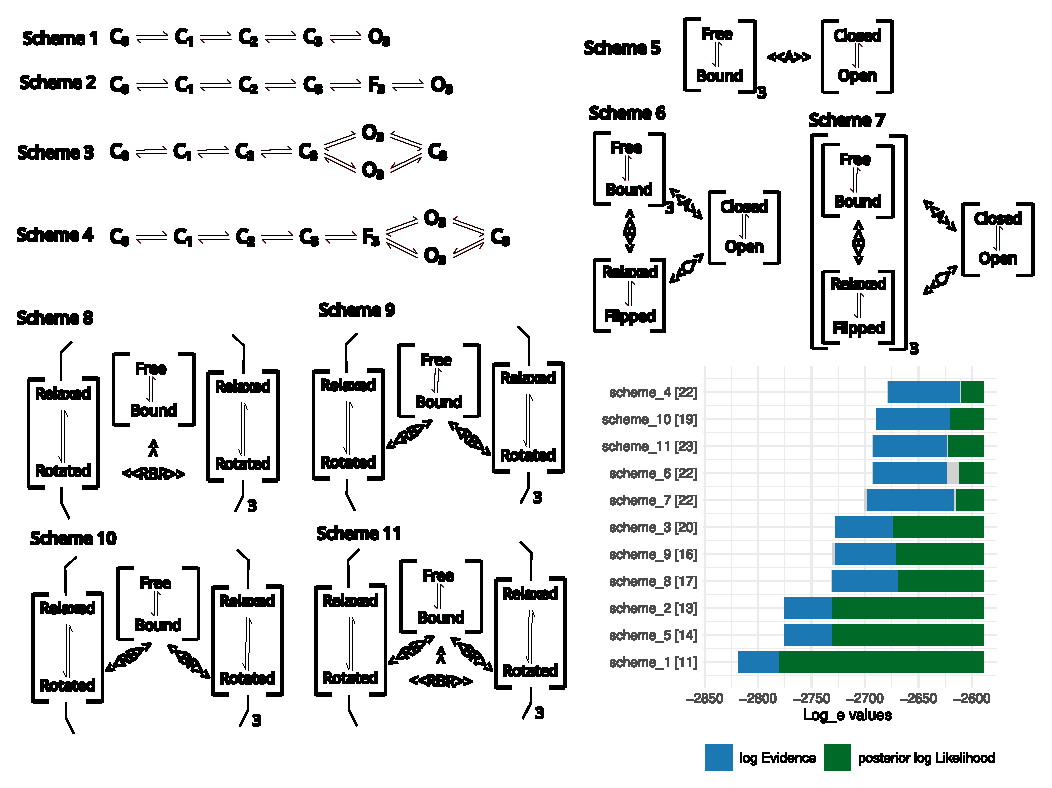
\includegraphics[width=1.0\textwidth]{Figure_1.eps}
\caption{Bayesian analysis of the tested kinetic schemes. For each tested kinetic scheme, the natural logarithm of the Evidence and posterior likelihood are indicated by the left end of the blue and green bars. Standard deviation of the samples are shown in light gray. Schemes are sorted according to their evidence, the highest at the top. Numbers in brackets next to the name of the schemes indicates the number of parameters. The length of the blue bar indicates the Kullback–Leibler divergence. }\label{fig_evidences}
\end{figure}



Highest Evidence was found for scheme 4 (\ref{fig_evidences}). That means that there still information in the kinetic responses that remains to be explained, Scheme 4 does not explain it until we found a reasonable mechanistic counterpart. 
Then, all all the remaining schemes the one with the highest evidence is scheme 10. This tell us that sequential asymmetric gating is the most likely mechanism. There is strong evidence against a symmetrical gating (10 vs 9) and there is evidence against a tertiary interaction with the other rotating subunit (10 vs 11). All the gating mechanism is explained by an asymmetric binding induced conformational change. No inter-subunit interaction is detected by the models. 
Also, there is strong evidence that supports this sequential asymmetric gating model against a synchronous gating model (scheme 6). 
However, a more sophisticated (and computationally prohibitive) synchronous diffusive process (where rotation is a continuous and possibly contagious process) cannot be discarded, so there is still some chance for a synchronous model. 




\subsection{posterior distribution of parameters of scheme 10: why is it bimodal}

\begin{figure}[h]
\centering
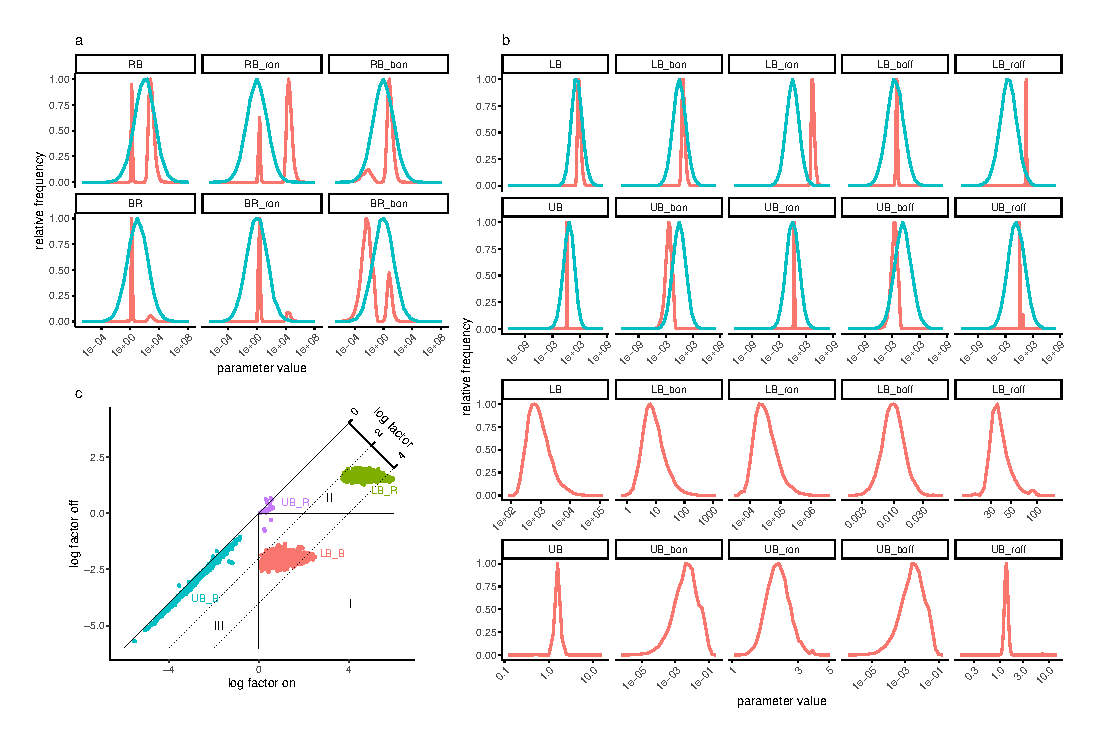
\includegraphics[width=1.0\textwidth]{Figure_2_ABC.eps}
\caption{Posterior distribution of allosteric parameters}\label{fig_bimodal}
\end{figure}


Schemes cannot mathematically differentiate between interaction with the left subunit or the right subunit, there is no left-right information in the macrocurrents. Therefore it is not surprising that the posterior distribution of the allosteric parameters of scheme 10 are all bimodal. As a way to break such symmetry in the priors we arbitrarily set BR to be 10 times RB. However, as the prior standard deviation of the $log10$ of both paramters (and all the remaining ones) was set to be 2, there was enough exploration at low thermodynamic temperatures to jump from one minimum to the other, so both values appear, although at different frequencies. 
This bimodality can be removed by determining which is greater if RB or BR, and if the former if the case, swap all the remaining parameters. In this was unimodal distribution were recovered for all allosteric parameters. 

\subsection{Asymmetry in the allosteric coupling. analysis of parameters, rates and states}
Once we correct for the bimodality we find that whereas one interaction is considerable (100-10E4 times), the other is much smaller(0-2 times). So, upon binding, there is a strong allosteric interaction with one subunit and a weak interaction with the other. This second subunit will have strong interaction at the other binding site that it is forming. 
If we then look at the decomposition of the allosteric interaction we see the following.
First, binding 




\subsection{ One path for activating, another for deactivating}

\subsection{white and pink noise}

\subsection{partial conductance and opening with two ATPs}


For simultaneous rotation of all subunits, this would not make much of a difference, so scheme 6 works the same for intra subunit binding sites or inter-subunit binding sites. 












%Sample body text. Sample body text. Sample body text. Sample body text. Sample body text. Sample body text. Sample body text. Sample body text.

%\section{This is an example for first level head---section head}\label{sec3}

%\subsection{This is an example for second level head---subsection head}\label{subsec2}

%\subsubsection{This is an example for third level head---subsubsection head}\label{subsubsec2}

%Sample body text. Sample body text. Sample body text. Sample body text. Sample body text. Sample body text. Sample body text. Sample body text. 

%\section{Equations}\label{sec4}

%Equations in \LaTeX\ can either be inline or on-a-line by itself (``display equations''). For
%inline equations use the \verb+$...$+ commands. E.g.: The equation
%$H\psi = E \psi$ is written via the command \verb+$H \psi = E \psi$+.

%For display equations (with auto generated equation numbers)
%one can use the equation or align environments:
%\begin{equation}
%\|\tilde{X}(k)\|^2 \leq\frac{\sum\limits_{i=1}^{p}\left\|\tilde{Y}_i(k)\right\|^2+\sum\limits_{j=1}^{q}\left\|\tilde{Z}_j(k)\right\|^2 }{p+q}.\label{eq1}
%\end{equation}
%where,
%\begin{align}
%D_\mu &=  \partial_\mu - ig \frac{\lambda^a}{2} A^a_\mu \nonumber \\
%F^a_{\mu\nu} &= \partial_\mu A^a_\nu - \partial_\nu A^a_\mu + g f^{abc} A^b_\mu A^a_\nu \label{eq2}
%\end{align}
%Notice the use of \verb+\nonumber+ in the align environment at the end
%of each line, except the last, so as not to produce equation numbers on
%lines where no equation numbers are required. The \verb+\label{}+ command
%should only be used at the last line of an align environment where
%\verb+\nonumber+ is not used.
%\begin{equation}
%Y_\infty = \left( \frac{m}{\textrm{GeV}} \right)^{-3}
%    \left[ 1 + \frac{3 \ln(m/\textrm{GeV})}{15}
%    + \frac{\ln(c_2/5)}{15} \right]
%\end{equation}
%The class file also supports the use of \verb+\mathbb{}+, \verb+\mathscr{}+ and
%\verb+\mathcal{}+ commands. As such \verb+\mathbb{R}+, \verb+\mathscr{R}+
%and \verb+\mathcal{R}+ produces $\mathbb{R}$, $\mathscr{R}$ and $\mathcal{R}$
%respectively (refer Subsubsection~\ref{subsubsec2}).

\section{Tables}\label{sec5}


\begin{table}[h]
\caption{Posterior distribution of scheme 10}\label{tab1}%
\begin{tabular}{@{}lllll@{}}
\toprule
 & parameters & median & CI\_hdi\_low & CI\_hdi\_hi \\ 
\midrule
1 & RB & 632.661 & 0.1441125 & 3.918861e+03 \\ 
  2 & RB\_ron & 2.454486e+04 & 1.260341 & 1.401152e+05 \\ 
  3 & RB\_bon & 6.248909 & 1.933688e-06 & 38.56124 \\ 
  4 & BR & 1.612385 & 0.2657464 & 1.106451e+03 \\ 
  5 & BR\_ron & 2.241492 & 1.077178 & 3.979711e+04 \\ 
  6 & BR\_bon & 6.986098e-03 & 9.626552e-07 & 11.16657 \\ 
\botrule
\end{tabular}
\footnotetext{Source: This is an example of table footnote. This is an example of table footnote.}
\footnotetext[1]{Example for a first table footnote. This is an example of table footnote.}
\footnotetext[2]{Example for a second table footnote. This is an example of table footnote.}
\end{table}







Tables can be inserted via the normal table and tabular environment. To put
footnotes inside tables you should use \verb+\footnotetext[]{...}+ tag.
The footnote appears just below the table itself (refer Tables~\ref{tab1} and \ref{tab2}). 
For the corresponding footnotemark use \verb+\footnotemark[...]+

\begin{table}[h]
\caption{Caption text}\label{tab1}%
\begin{tabular}{@{}llll@{}}
\toprule
Column 1 & Column 2  & Column 3 & Column 4\\
\midrule
row 1    & data 1   & data 2  & data 3  \\
row 2    & data 4   & data 5\footnotemark[1]  & data 6  \\
row 3    & data 7   & data 8  & data 9\footnotemark[2]  \\
\botrule
\end{tabular}
\footnotetext{Source: This is an example of table footnote. This is an example of table footnote.}
\footnotetext[1]{Example for a first table footnote. This is an example of table footnote.}
\footnotetext[2]{Example for a second table footnote. This is an example of table footnote.}
\end{table}

\noindent
The input format for the above table is as follows:


%\iffalse

%%=============================================%%
%% For presentation purpose, we have included  %%
%% \bigskip command. Please ignore this.       %%
%%=============================================%%
\bigskip
\begin{verbatim}
\begin{table}[<placement-specifier>]
\caption{<table-caption>}\label{<table-label>}%
\begin{tabular}{@{}llll@{}}
\toprule
Column 1 & Column 2 & Column 3 & Column 4\\
\midrule
row 1 & data 1 & data 2	 & data 3 \\
row 2 & data 4 & data 5\footnotemark[1] & data 6 \\
row 3 & data 7 & data 8	 & data 9\footnotemark[2]\\
\botrule
\end{tabular}
\footnotetext{Source: This is an example of table footnote. 
This is an example of table footnote.}
\footnotetext[1]{Example for a first table footnote.
This is an example of table footnote.}
\footnotetext[2]{Example for a second table footnote. 
This is an example of table footnote.}
\end{table}
\end{verbatim}
\bigskip
%%=============================================%%
%% For presentation purpose, we have included  %%
%% \bigskip command. Please ignore this.       %%
%%=============================================%%


\begin{table}[h]
\caption{Example of a lengthy table which is set to full textwidth}\label{tab2}
\begin{tabular*}{\textwidth}{@{\extracolsep\fill}lcccccc}
\toprule%
& \multicolumn{3}{@{}c@{}}{Element 1\footnotemark[1]} & \multicolumn{3}{@{}c@{}}{Element 2\footnotemark[2]} \\\cmidrule{2-4}\cmidrule{5-7}%
Project & Energy & $\sigma_{calc}$ & $\sigma_{expt}$ & Energy & $\sigma_{calc}$ & $\sigma_{expt}$ \\
\midrule
Element 3  & 990 A & 1168 & $1547\pm12$ & 780 A & 1166 & $1239\pm100$\\
Element 4  & 500 A & 961  & $922\pm10$  & 900 A & 1268 & $1092\pm40$\\
\botrule
\end{tabular*}
\footnotetext{Note: This is an example of table footnote. This is an example of table footnote this is an example of table footnote this is an example of~table footnote this is an example of table footnote.}
\footnotetext[1]{Example for a first table footnote.}
\footnotetext[2]{Example for a second table footnote.}
\end{table}

In case of double column layout, tables which do not fit in single column width should be set to full text width. For this, you need to use \verb+\begin{table*}+ \verb+...+ \verb+\end{table*}+ instead of \verb+\begin{table}+ \verb+...+ \verb+\end{table}+ environment. Lengthy tables which do not fit in textwidth should be set as rotated table. For this, you need to use \verb+\begin{sidewaystable}+ \verb+...+ \verb+\end{sidewaystable}+ instead of \verb+\begin{table*}+ \verb+...+ \verb+\end{table*}+ environment. This environment puts tables rotated to single column width. For tables rotated to double column width, use \verb+\begin{sidewaystable*}+ \verb+...+ \verb+\end{sidewaystable*}+.

\begin{sidewaystable}
\caption{Tables which are too long to fit, should be written using the ``sidewaystable'' environment as shown here}\label{tab3}
\begin{tabular*}{\textheight}{@{\extracolsep\fill}lcccccc}
\toprule%
& \multicolumn{3}{@{}c@{}}{Element 1\footnotemark[1]}& \multicolumn{3}{@{}c@{}}{Element\footnotemark[2]} \\\cmidrule{2-4}\cmidrule{5-7}%
Projectile & Energy	& $\sigma_{calc}$ & $\sigma_{expt}$ & Energy & $\sigma_{calc}$ & $\sigma_{expt}$ \\
\midrule
Element 3 & 990 A & 1168 & $1547\pm12$ & 780 A & 1166 & $1239\pm100$ \\
Element 4 & 500 A & 961  & $922\pm10$  & 900 A & 1268 & $1092\pm40$ \\
Element 5 & 990 A & 1168 & $1547\pm12$ & 780 A & 1166 & $1239\pm100$ \\
Element 6 & 500 A & 961  & $922\pm10$  & 900 A & 1268 & $1092\pm40$ \\
\botrule
\end{tabular*}
\footnotetext{Note: This is an example of table footnote this is an example of table footnote this is an example of table footnote this is an example of~table footnote this is an example of table footnote.}
\footnotetext[1]{This is an example of table footnote.}
\end{sidewaystable}

\section{Figures}\label{sec6}

As per the \LaTeX\ standards you need to use eps images for \LaTeX\ compilation and \verb+pdf/jpg/png+ images for \verb+PDFLaTeX+ compilation. This is one of the major difference between \LaTeX\ and \verb+PDFLaTeX+. Each image should be from a single input .eps/vector image file. Avoid using subfigures. The command for inserting images for \LaTeX\ and \verb+PDFLaTeX+ can be generalized. The package used to insert images in \verb+LaTeX/PDFLaTeX+ is the graphicx package. Figures can be inserted via the normal figure environment as shown in the below example:

%%=============================================%%
%% For presentation purpose, we have included  %%
%% \bigskip command. Please ignore this.       %%
%%=============================================%%
\bigskip
\begin{verbatim}
\begin{figure}[<placement-specifier>]
\centering
\includegraphics{<eps-file>}
\caption{<figure-caption>}\label{<figure-label>}
\end{figure}
\end{verbatim}
\bigskip
%%=============================================%%
%% For presentation purpose, we have included  %%
%% \bigskip command. Please ignore this.       %%
%%=============================================%%


\begin{figure}[h]
\centering
\includegraphics[width=0.9\textwidth]{fig.eps}
\caption{This is a widefig. This is an example of long caption this is an example of long caption  this is an example of long caption this is an example of long caption}\label{fig1}
\end{figure}

In case of double column layout, the above format puts figure captions/images to single column width. To get spanned images, we need to provide \verb+\begin{figure*}+ \verb+...+ \verb+\end{figure*}+.

For sample purpose, we have included the width of images in the optional argument of \verb+\includegraphics+ tag. Please ignore this. 

\section{Algorithms, Program codes and Listings}\label{sec7}

Packages \verb+algorithm+, \verb+algorithmicx+ and \verb+algpseudocode+ are used for setting algorithms in \LaTeX\ using the format:

%%=============================================%%
%% For presentation purpose, we have included  %%
%% \bigskip command. Please ignore this.       %%
%%=============================================%%
\bigskip
\begin{verbatim}
\begin{algorithm}
\caption{<alg-caption>}\label{<alg-label>}
\begin{algorithmic}[1]
. . .
\end{algorithmic}
\end{algorithm}
\end{verbatim}
\bigskip
%%=============================================%%
%% For presentation purpose, we have included  %%
%% \bigskip command. Please ignore this.       %%
%%=============================================%%

You may refer above listed package documentations for more details before setting \verb+algorithm+ environment. For program codes, the ``verbatim'' package is required and the command to be used is \verb+\begin{verbatim}+ \verb+...+ \verb+\end{verbatim}+. 

Similarly, for \verb+listings+, use the \verb+listings+ package. \verb+\begin{lstlisting}+ \verb+...+ \verb+\end{lstlisting}+ is used to set environments similar to \verb+verbatim+ environment. Refer to the \verb+lstlisting+ package documentation for more details.

A fast exponentiation procedure:

\lstset{texcl=true,basicstyle=\small\sf,commentstyle=\small\rm,mathescape=true,escapeinside={(*}{*)}}
\begin{lstlisting}
begin
  for $i:=1$ to $10$ step $1$ do
      expt($2,i$);  
      newline() od                (*\textrm{Comments will be set flush to the right margin}*)
where
proc expt($x,n$) $\equiv$
  $z:=1$;
  do if $n=0$ then exit fi;
     do if odd($n$) then exit fi;                 
        comment: (*\textrm{This is a comment statement;}*)
        $n:=n/2$; $x:=x*x$ od;
     { $n>0$ };
     $n:=n-1$; $z:=z*x$ od;
  print($z$). 
end
\end{lstlisting}

\begin{algorithm}
\caption{Calculate $y = x^n$}\label{algo1}
\begin{algorithmic}[1]
\Require $n \geq 0 \vee x \neq 0$
\Ensure $y = x^n$ 
\State $y \Leftarrow 1$
\If{$n < 0$}\label{algln2}
        \State $X \Leftarrow 1 / x$
        \State $N \Leftarrow -n$
\Else
        \State $X \Leftarrow x$
        \State $N \Leftarrow n$
\EndIf
\While{$N \neq 0$}
        \If{$N$ is even}
            \State $X \Leftarrow X \times X$
            \State $N \Leftarrow N / 2$
        \Else[$N$ is odd]
            \State $y \Leftarrow y \times X$
            \State $N \Leftarrow N - 1$
        \EndIf
\EndWhile
\end{algorithmic}
\end{algorithm}

%%=============================================%%
%% For presentation purpose, we have included  %%
%% \bigskip command. Please ignore this.       %%
%%=============================================%%
\bigskip
\begin{minipage}{\hsize}%
\lstset{frame=single,framexleftmargin=-1pt,framexrightmargin=-17pt,framesep=12pt,linewidth=0.98\textwidth,language=pascal}% Set your language (you can change the language for each code-block optionally)
%%% Start your code-block
\begin{lstlisting}
for i:=maxint to 0 do
begin
{ do nothing }
end;
Write('Case insensitive ');
Write('Pascal keywords.');
\end{lstlisting}
\end{minipage}

\section{Cross referencing}\label{sec8}

Environments such as figure, table, equation and align can have a label
declared via the \verb+\label{#label}+ command. For figures and table
environments use the \verb+\label{}+ command inside or just
below the \verb+\caption{}+ command. You can then use the
\verb+\ref{#label}+ command to cross-reference them. As an example, consider
the label declared for Figure~\ref{fig1} which is
\verb+\label{fig1}+. To cross-reference it, use the command 
\verb+Figure \ref{fig1}+, for which it comes up as
``Figure~\ref{fig1}''. 

To reference line numbers in an algorithm, consider the label declared for the line number 2 of Algorithm~\ref{algo1} is \verb+\label{algln2}+. To cross-reference it, use the command \verb+\ref{algln2}+ for which it comes up as line~\ref{algln2} of Algorithm~\ref{algo1}.

\subsection{Details on reference citations}\label{subsec7}

Standard \LaTeX\ permits only numerical citations. To support both numerical and author-year citations this template uses \verb+natbib+ \LaTeX\ package. For style guidance please refer to the template user manual.

Here is an example for \verb+\cite{...}+: \cite{bib1}. Another example for \verb+\citep{...}+: \citep{bib2}. For author-year citation mode, \verb+\cite{...}+ prints Jones et al. (1990) and \verb+\citep{...}+ prints (Jones et al., 1990).

All cited bib entries are printed at the end of this article: \cite{bib3}, \cite{bib4}, \cite{bib5}, \cite{bib6}, \cite{bib7}, \cite{bib8}, \cite{bib9}, \cite{bib10}, \cite{bib11}, \cite{bib12} and \cite{bib13}.


\section{Examples for theorem like environments}\label{sec10}

For theorem like environments, we require \verb+amsthm+ package. There are three types of predefined theorem styles exists---\verb+thmstyleone+, \verb+thmstyletwo+ and \verb+thmstylethree+ 

%%=============================================%%
%% For presentation purpose, we have included  %%
%% \bigskip command. Please ignore this.       %%
%%=============================================%%
\bigskip
\begin{tabular}{|l|p{19pc}|}
\hline
\verb+thmstyleone+ & Numbered, theorem head in bold font and theorem text in italic style \\\hline
\verb+thmstyletwo+ & Numbered, theorem head in roman font and theorem text in italic style \\\hline
\verb+thmstylethree+ & Numbered, theorem head in bold font and theorem text in roman style \\\hline
\end{tabular}
\bigskip
%%=============================================%%
%% For presentation purpose, we have included  %%
%% \bigskip command. Please ignore this.       %%
%%=============================================%%

For mathematics journals, theorem styles can be included as shown in the following examples:

\begin{theorem}[Theorem subhead]\label{thm1}
Example theorem text. Example theorem text. Example theorem text. Example theorem text. Example theorem text. 
Example theorem text. Example theorem text. Example theorem text. Example theorem text. Example theorem text. 
Example theorem text. 
\end{theorem}

Sample body text. Sample body text. Sample body text. Sample body text. Sample body text. Sample body text. Sample body text. Sample body text.

\begin{proposition}
Example proposition text. Example proposition text. Example proposition text. Example proposition text. Example proposition text. 
Example proposition text. Example proposition text. Example proposition text. Example proposition text. Example proposition text. 
\end{proposition}

Sample body text. Sample body text. Sample body text. Sample body text. Sample body text. Sample body text. Sample body text. Sample body text.

\begin{example}
Phasellus adipiscing semper elit. Proin fermentum massa
ac quam. Sed diam turpis, molestie vitae, placerat a, molestie nec, leo. Maecenas lacinia. Nam ipsum ligula, eleifend
at, accumsan nec, suscipit a, ipsum. Morbi blandit ligula feugiat magna. Nunc eleifend consequat lorem. 
\end{example}

Sample body text. Sample body text. Sample body text. Sample body text. Sample body text. Sample body text. Sample body text. Sample body text.

\begin{remark}
Phasellus adipiscing semper elit. Proin fermentum massa
ac quam. Sed diam turpis, molestie vitae, placerat a, molestie nec, leo. Maecenas lacinia. Nam ipsum ligula, eleifend
at, accumsan nec, suscipit a, ipsum. Morbi blandit ligula feugiat magna. Nunc eleifend consequat lorem. 
\end{remark}

Sample body text. Sample body text. Sample body text. Sample body text. Sample body text. Sample body text. Sample body text. Sample body text.

\begin{definition}[Definition sub head]
Example definition text. Example definition text. Example definition text. Example definition text. Example definition text. Example definition text. Example definition text. Example definition text. 
\end{definition}

Additionally a predefined ``proof'' environment is available: \verb+\begin{proof}+ \verb+...+ \verb+\end{proof}+. This prints a ``Proof'' head in italic font style and the ``body text'' in roman font style with an open square at the end of each proof environment. 

\begin{proof}
Example for proof text. Example for proof text. Example for proof text. Example for proof text. Example for proof text. Example for proof text. Example for proof text. Example for proof text. Example for proof text. Example for proof text. 
\end{proof}

Sample body text. Sample body text. Sample body text. Sample body text. Sample body text. Sample body text. Sample body text. Sample body text.

\begin{proof}[Proof of Theorem~{\upshape\ref{thm1}}]
Example for proof text. Example for proof text. Example for proof text. Example for proof text. Example for proof text. Example for proof text. Example for proof text. Example for proof text. Example for proof text. Example for proof text. 
\end{proof}

\noindent
For a quote environment, use \verb+\begin{quote}...\end{quote}+
\begin{quote}
Quoted text example. Aliquam porttitor quam a lacus. Praesent vel arcu ut tortor cursus volutpat. In vitae pede quis diam bibendum placerat. Fusce elementum
convallis neque. Sed dolor orci, scelerisque ac, dapibus nec, ultricies ut, mi. Duis nec dui quis leo sagittis commodo.
\end{quote}

Sample body text. Sample body text. Sample body text. Sample body text. Sample body text (refer Figure~\ref{fig1}). Sample body text. Sample body text. Sample body text (refer Table~\ref{tab3}). 







\textbf{Ethical approval declarations} (only required where applicable) Any article reporting experiment/s carried out on (i)~live vertebrate (or higher invertebrates), (ii)~humans or (iii)~human samples must include an unambiguous statement within the methods section that meets the following requirements: 

\begin{enumerate}[1.]
\item Approval: a statement which confirms that all experimental protocols were approved by a named institutional and/or licensing committee. Please identify the approving body in the methods section

\item Accordance: a statement explicitly saying that the methods were carried out in accordance with the relevant guidelines and regulations

\item Informed consent (for experiments involving humans or human tissue samples): include a statement confirming that informed consent was obtained from all participants and/or their legal guardian/s
\end{enumerate}

If your manuscript includes potentially identifying patient/participant information, or if it describes human transplantation research, or if it reports results of a clinical trial then  additional information will be required. Please visit (\url{https://www.nature.com/nature-research/editorial-policies}) for Nature Portfolio journals, (\url{https://www.springer.com/gp/authors-editors/journal-author/journal-author-helpdesk/publishing-ethics/14214}) for Springer Nature journals, or (\url{https://www.biomedcentral.com/getpublished/editorial-policies\#ethics+and+consent}) for BMC.

\fi

\section{Discussion}\label{sec12}

Discussions should be brief and focused. In some disciplines use of Discussion or `Conclusion' is interchangeable. It is not mandatory to use both. Some journals prefer a section `Results and Discussion' followed by a section `Conclusion'. Please refer to Journal-level guidance for any specific requirements. 

\section{Conclusion}\label{sec13}

Conclusions may be used to restate your hypothesis or research question, restate your major findings, explain the relevance and the added value of your work, highlight any limitations of your study, describe future directions for research and recommendations. 

In some disciplines use of Discussion or 'Conclusion' is interchangeable. It is not mandatory to use both. Please refer to Journal-level guidance for any specific requirements. 

\backmatter

\bmhead{Supplementary information}

If your article has accompanying supplementary file/s please state so here. 

Authors reporting data from electrophoretic gels and blots should supply the full unprocessed scans for key as part of their Supplementary information. This may be requested by the editorial team/s if it is missing.

Please refer to Journal-level guidance for any specific requirements.

\bmhead{Acknowledgements}


Acknowledgements are not compulsory. Where included they should be brief. Grant or contribution numbers may be acknowledged.

Please refer to Journal-level guidance for any specific requirements.

\section*{Declarations}

Some journals require declarations to be submitted in a standardised format. Please check the Instructions for Authors of the journal to which you are submitting to see if you need to complete this section. If yes, your manuscript must contain the following sections under the heading `Declarations':

\begin{itemize}
\item Funding
\item Conflict of interest/Competing interests (check journal-specific guidelines for which heading to use)
\item Ethics approval and consent to participate
\item Consent for publication
\item Data availability 
\item Materials availability
\item Code availability 
\item Author contribution
\end{itemize}

\noindent
If any of the sections are not relevant to your manuscript, please include the heading and write `Not applicable' for that section. 

%%===================================================%%
%% For presentation purpose, we have included        %%
%% \bigskip command. Please ignore this.             %%
%%===================================================%%
\bigskip
\begin{flushleft}%
Editorial Policies for:

\bigskip\noindent
Springer journals and proceedings: \url{https://www.springer.com/gp/editorial-policies}

\bigskip\noindent
Nature Portfolio journals: \url{https://www.nature.com/nature-research/editorial-policies}

\bigskip\noindent
\textit{Scientific Reports}: \url{https://www.nature.com/srep/journal-policies/editorial-policies}

\bigskip\noindent
BMC journals: \url{https://www.biomedcentral.com/getpublished/editorial-policies}
\end{flushleft}

\begin{appendices}

\section{Section title of first appendix}\label{secA1}

An appendix contains supplementary information that is not an essential part of the text itself but which may be helpful in providing a more comprehensive understanding of the research problem or it is information that is too cumbersome to be included in the body of the paper.

%%=============================================%%
%% For submissions to Nature Portfolio Journals %%
%% please use the heading ``Extended Data''.   %%
%%=============================================%%

%%=============================================================%%
%% Sample for another appendix section			       %%
%%=============================================================%%

%% \section{Example of another appendix section}\label{secA2}%
%% Appendices may be used for helpful, supporting or essential material that would otherwise 
%% clutter, break up or be distracting to the text. Appendices can consist of sections, figures, 
%% tables and equations etc.

\end{appendices}

%%===========================================================================================%%
%% If you are submitting to one of the Nature Portfolio journals, using the eJP submission   %%
%% system, please include the references within the manuscript file itself. You may do this  %%
%% by copying the reference list from your .bbl file, paste it into the main manuscript .tex %%
%% file, and delete the associated \verb+\bibliography+ commands.                            %%
%%===========================================================================================%%

\bibliography{biblio}% common bib file
%% if required, the content of .bbl file can be included here once bbl is generated
%%\input sn-article.bbl


\end{document}
